\documentclass[11pt]{article}
\usepackage[T1]{fontenc}
\usepackage{lmodern}
\usepackage[margin=0.93in]{geometry}
\usepackage{amsmath,amssymb,amsthm,mathtools}
\usepackage{microtype}
\usepackage{booktabs}
\usepackage{enumitem}
\usepackage{tikz}
\usetikzlibrary{arrows.meta,positioning,fit,backgrounds}
\usepackage[colorlinks=true,linkcolor=blue!45!black,citecolor=blue!45!black,urlcolor=blue!45!black]{hyperref}
\hypersetup{pdftitle={Simulating One-Tape Time in Two-Fifths-Power Space},pdfauthor={OpenAI}}
\setlength{\emergencystretch}{2em}
\setlist{topsep=4pt,itemsep=2pt}
\newtheorem{theorem}{Theorem}
\newtheorem{lemma}[theorem]{Lemma}
\newtheorem{proposition}[theorem]{Proposition}
\newtheorem{corollary}[theorem]{Corollary}
\theoremstyle{definition}
\newtheorem{definition}[theorem]{Definition}
\theoremstyle{remark}
\newtheorem{remark}[theorem]{Remark}
\newcommand{\bits}{\{0,1\}}
\newcommand{\F}{\mathbb F}
\newcommand{\polylog}{\operatorname{polylog}}
\newcommand{\Add}{\mathsf{Add}}
\newcommand{\wt}{\operatorname{wt}}
\newcommand{\softO}{\widetilde O}
\title{Simulating One-Tape Time in Two-Fifths-Power Space}
\author{OpenAI}
\date{September 25, 2026}
\begin{document}
\maketitle
\begin{abstract}
We show that a fixed deterministic Turing machine with one writable tape and
head can be simulated in \(O(T^{2/5}\polylog(T+2))\) work-space bits when a
binary time cap \(T\ge2\) is supplied. The simulator computes the finite-control
and halting outcome by time \(T\); its running time is unrestricted. The result
allows a fixed number of read-only input heads and requires a fixed accessor
that supplies every initial writable and read-only symbol within distance
\(T\) of the relevant head origin in polylogarithmic space. This improves the square-root
space exponent for one-tape machines, answering Williams's question for this model.
\end{abstract}
\section{Introduction}
\label{sec:introduction}

How much work space is needed to reproduce a time-bounded computation
when the simulator may take arbitrarily long?
The classical one-read/write-tape \(O(\sqrt t)\) simulation is attributed
to Hopcroft and Ullman in Williams's account~\cite[Section~2.1]{Williams2025}.
Related work studied time--space tradeoffs for single-tape and offline
Turing machines~\cite{Paterson1972,IbarraMoran1983,LiskiewiczLorys1990}.
We use the supplied-cap model stated below.
Williams proved that deterministic multitape time \(t(n)\), for
\(t(n)\ge n\), can be simulated in
\(O(\sqrt{t(n)\log t(n)})\) space~\cite[Theorem~1.1]{Williams2025}.
His proof uses the additive dependence on value length and tree height
in the tree-evaluation algorithm of Cook and Mertz~\cite[Theorem~7]{CookMertz2024}.
Goldreich's 2024 exposition explains this algorithm through univariate
interpolation and global storage~\cite{Goldreich2024}.
In Section~5 of his full version, Williams asks whether the classical
square-root space exponent for \emph{one-tape} machines can be reduced
by a fixed positive constant. We answer this question affirmatively for
the model below.

\paragraph{Model and output.}
The simulated machine is fixed and deterministic, with a finite state
set and finite alphabet. It has one writable tape, indexed by the
integers, with one head; a transition reads and writes the current cell
and then moves that head by at most one position.
A fixed number of additional read-only input heads may move by at most
one position per step. All heads start at fixed origins.
The writable tape initially contains the input in the usual fixed
encoding, or is blank with the input on a separate read-only tape.
The following uniform interface also permits other initial encodings.
For the initial writable tape and for each read-only head, let a fixed
tag \(h\) identify its symbol source and starting origin. Write
\(\sigma_h(x,q)\) for the symbol at displacement \(q\) from that
origin on public input \(x\). Tags for heads on the same tape refer to
the same underlying contents, with the corresponding coordinate shifts.
These symbol functions are fixed independently of every cap.

Fix one deterministic accessor \(\mathsf{Sym}\) and constants
\(C_0,C_1\ge1\). We say that the \emph{access condition holds for \((x,T)\)}
if, for every tag \(h\) and integer \(|q|\le T\),
\(\mathsf{Sym}(x,h,T,q)\) halts with \(\sigma_h(x,q)\) using at most
\(C_0\log^{C_1}(T+2)\) work-space bits. The program and constants are
independent of \(x,T,q\), with dependence allowed on the fixed machine
and symbol interface. The condition covers every coordinate in the
numerical range, including coordinates inspected by proposed local
computations. A capped invocation assumes it only for its own pair
\((x,T)\). Ordinary input access satisfies it for every cap by storing
the requested coordinate and rescanning to that position or an endmarker.

The simulator is given the original input and a binary time cap \(T\).
The simulator and accessor use ordinary endmarked read-only access to
the public input, with the input head confined between the endmarkers.
The simulator's output is the finite-control and halting
outcome after at most \(T\) simulated steps, with halting states made
absorbing. Input storage is not charged to work space. The simulator
does not have to store the entire final tape.
All space bounds count bits; constants may depend on the fixed machine
and accessor.
We write \(\softO(f(T))\) for
\(O(f(T)\log^C(T+2))\), with a fixed constant \(C\).

\begin{theorem}
\label{thm:main}
Fix a deterministic machine with one writable tape and head, a fixed
number of read-only input heads, unit movement and fixed origins for
all heads, cap-independent symbol functions, and a fixed accessor as above.
For every public input \(x\) and supplied binary cap \(T\ge2\) for which
the access condition
holds, its finite-control and halting outcome by time \(T\) can be
computed deterministically in \(\softO(T^{2/5})\) work-space bits,
excluding storage for the read-only input. Simulation time is
unrestricted, and the final writable tape need not be materialized.
If the access condition holds for \((x,T)\) at every \(T\ge2\), and
the machine halts on \(x\) after \(t\) steps without a supplied running
time, its outcome can be computed in
\(\softO((t+2)^{2/5})\) work-space bits.
\end{theorem}

The ordinary one-sided one-tape decision model is included: the machine
can enforce a left boundary, ordinary input symbols are obtained by
rescanning, and acceptance or rejection is part of finite control.
In particular, every fixed exponent \(\epsilon>2/5\) suffices.
For any fixed \(0<\delta<1/10\), the bound in
Theorem~\ref{thm:main} is \(O(T^{1/2-\delta})\), as requested by
Williams's one-tape question. No log-free endpoint at exponent \(2/5\)
is asserted. The result applies to one writable head, even when
additional read-only input heads are present; it is not a two-fifths
bound for arbitrary multitape machines.
Section~\ref{sec:multitape} gives a separate
\(\softO(\sqrt T)\) simulation for every fixed number of writable tapes.

\paragraph{The mechanism.}
Choose a shifted partition of the writable tape into blocks of width
\(b\). One offset has only \(O(T/b)\) block visits.
A visit accesses one long block and exchanges only a short controller,
consisting of the state, head positions, time and terminal flags.
Once a proposed controller transcript is fixed, all visits to a
particular block can be replayed using that block's initial contents.
Consistency of the transcript therefore factors over the blocks.

Group \(b\) visits into an epoch and append their controllers in rounds
of \(k=\sqrt b\) visits. The complete history and one block each fit in
\(\softO(b)\) bits. Interpolation evaluates a history update while
keeping the round guess out of the recursive calls to the preceding
history. A guess is retained only on a call to an epoch-start block.
Such a call immediately leads to earlier epochs, so a recursion path
pays for at most one retained round guess per epoch.
The resulting space bound is
\[
 \softO\!\left(b+(1+T/b^2)\sqrt b\right),
\]
balanced at \(b\asymp T^{2/5}\).

The reusable ingredient is Lemma~\ref{lem:weighted-evaluation}:
factored word recurrences can be evaluated with one fixed register
pool and an ordinary stack charged by the sizes of suspended guesses.
It supplies an additive translation of a true word from arbitrary
initial register contents and restores every other register.
This permits descendants to borrow the caller's inputs and partially
accumulated output. The use of shared storage follows the
Cook--Mertz approach, with the interpolation viewpoint explained also
by Goldreich~\cite{CookMertz2024,Goldreich2024}; the factored round rule
and its placement within the epoch dependencies produce the space
estimate above.
We prove the required evaluator directly, including its local
computation and stack costs.

\paragraph{Limits.}
Theorem~\ref{thm:main} concerns space, with no useful bound on simulation
time. It cannot be iterated as a time improvement.
The parameter calculation in Section~\ref{sec:balance} explains why
changing the three scales in this construction alone does not lower
its exponent. It is not a lower bound on other simulations, an
optimality claim, or a claim of a general multitape improvement.

\section{An evaluator with weighted dependency paths}\label{sec:evaluation}

We prove the arithmetic evaluation result used below.  Its procedure adds a
scalar multiple of a word's fixed augmented value to one chosen register and
restores every other register, from arbitrary contents on entry.  A caller can
therefore leave its inputs and partial output in a shared pool while a child
borrows the same registers.  The remaining stack cost depends on the
dependency followed: a large loop index is saved only on designated edges.
The translation and interpolation method is related to space-efficient tree
evaluation and its global-storage exposition~\cite{CookMertz2024,Goldreich2024}; all the algebra, register invariants, and
uniformity needed here are proved explicitly.

Throughout this section, $T\ge2$, a word has a common padded width $d\ge1$,
and $r$ is a fixed constant.  A polynomial bound means a bound by $T^C$ for a
fixed constant $C$.  The notation $\polylog T$ permits fixed powers of
$\log(T+2)$, with constants depending on the uniform algorithms under
consideration.  For $v\in\bits^d$, write
\[
 \overline v=(v_1,\ldots,v_d,1).
\]
The last coordinate of an arbitrary vector $z\in\F^{d+1}$ is denoted $z_*$;
it need not equal $1$.

\begin{lemma}[Uniform fields]\label{lem:field}
Given an integer $\Delta\ge1$ bounded polynomially in $T$, one can uniformly
construct a field $\F$ of characteristic two with $|\F|>\Delta$.  Field
elements have $O(\log T)$ bits.  A description of the field, enumeration of its
elements, its arithmetic, and inversion of nonzero elements all require
$\polylog T$ space.
\end{lemma}
\begin{proof}
Start with $\mathbb F_2$.  In a finite field $K$ of characteristic two, the
additive map $x\mapsto x^2+x$ has kernel $\{0,1\}$, since
$x^2+x=x(x+1)$.  Its image therefore contains exactly half of $K$.
Enumerate $a\in K$, and, for each candidate, enumerate $x\in K$ to test
whether $a=x^2+x$.  An $a$ outside the image exists.  The polynomial
$X^2+X+a$ has no root in $K$, hence is irreducible, and
\[
 K[X]/(X^2+X+a)
\]
is a field: the Euclidean algorithm gives an inverse modulo this polynomial
for every nonzero residue of degree less than two.  Its elements are pairs
of elements of $K$ and its cardinality is $|K|^2$.

Repeat until the cardinality first exceeds $\Delta$.  The final cardinality
is at most $\max(2,\Delta^2)$, and its binary vector representation has
$m=O(\log T)$ bits.  The selected coefficients at all levels together use
$O(m)$ bits, since their representation lengths form a geometric sequence.
Arithmetic can be implemented recursively on the pairs, reducing products
using the defining quadratics.  A direct recursive implementation uses at
most a polynomial in $m$ space; its recursion depth is $O(\log m)$.
Enumeration uses an $m$-bit counter.  Alternatively, once multiplication is
available, inversion can be implemented simply by enumerating all elements
until their product with the given nonzero element is $1$.  The searches for
the extension coefficients have the same space bound.  No time bound is
required.
\end{proof}

\begin{lemma}[Homogeneous lookup extensions]\label{lem:homogenization}
For every total function $f:(\bits^d)^a\to\bits$, where $a$ is fixed,
there is a polynomial $\widetilde f$ on $(\F^{d+1})^a$ that agrees with $f$
on augmented Boolean arguments and is homogeneous of degree $d$ separately
in every argument.  If a coordinate of $f$ is computable in
$O(d\polylog T)$ space from its Boolean arguments, its extension can be
evaluated at supplied field vectors in that space, with no recursive word
evaluation.  The same statement applies coordinatewise to augmented
word-valued functions.
\end{lemma}
\begin{proof}
For $u\in\bits^d$ and $z\in\F^{d+1}$, set
\begin{equation}\label{eq:homogeneous-basis}
 B_u(z)=\prod_{\ell=1}^d
 \begin{cases}
  z_\ell,&u_\ell=1,\\
  z_*-z_\ell,&u_\ell=0.
 \end{cases}
\end{equation}
At $z=\overline v$, this is $1$ for $u=v$ and $0$ otherwise.  Thus
\begin{equation}\label{eq:lookup-extension}
 \widetilde f(z^{(1)},\ldots,z^{(a)})
 =\sum_{u^{(1)},\ldots,u^{(a)}\in\bits^d}
 f(u^{(1)},\ldots,u^{(a)})
 \prod_{j=1}^a B_{u^{(j)}}(z^{(j)})
\end{equation}
has the stated agreement and homogeneity.  The zero polynomial is allowed
as a homogeneous polynomial of the indicated degree.  For a word output,
apply the formula to each of its $d$ bit coordinates and to its extra
coordinate, whose Boolean value is $1$.

To evaluate one coordinate, enumerate the $a$ Boolean assignments, compute
the corresponding Boolean function value, and compute the basis products
and running sum using field scalars.  The assignments occupy $ad=O(d)$ bits;
the local Boolean computation occupies $O(d\polylog T)$ bits.  All inputs
are the supplied vectors, read without modification, and immutable
parameters.  This routine makes no
calls to evaluate any word.  Its entire temporary storage can be discarded
when its scalar result has been obtained.
\end{proof}

The augmentation of constant functions is essential.  From
\eqref{eq:homogeneous-basis},
\[
 \sum_{u\in\bits^d}B_u(z)=z_*^d.
\]
Consequently the extension of a globally constant-one one-word function is
$z_*^d$, and that of a globally constant-one two-word function is
$h_*^d a_*^d$.  Neither is replaced by literal $1$.  Moreover, a predicate
that happens to be true for every array value at one particular Boolean
history need not be globally constant.  Such a predicate retains its full
lookup extension.  In particular, the following argument uses these
polynomials even when a shifted augmentation coordinate is zero.

\begin{lemma}[Top-coefficient extraction]\label{lem:top-coefficient}
Let $L$ be an integer with $0\le L<|\F|$, choose any $L+1$ distinct
elements $S_L\subseteq\F$, and set
\[
 \omega_L(s)=\left(\prod_{u\in S_L\setminus\{s\}}(s-u)\right)^{-1}
 \qquad(s\in S_L).
\]
For every univariate polynomial $p$ of degree at most $L$,
\begin{equation}\label{eq:top-coefficient}
 [X^L]p(X)=\sum_{s\in S_L}\omega_L(s)p(s).
\end{equation}
If $Q$ is homogeneous of degree $L$, then, for arbitrary field vectors $a,v$,
\begin{equation}\label{eq:translation-extraction}
 \sum_{s\in S_L}\omega_L(s)Q(a+sv)=Q(v).
\end{equation}
Choosing $S_L$ as the first $L+1$ elements in the uniform field enumeration,
its points and weights can be enumerated and recomputed in $\polylog T$
space when $L$ is polynomially bounded in $T$.
\end{lemma}
\begin{proof}
The polynomials
\[
 \prod_{u\in S_L\setminus\{s\}}\frac{X-u}{s-u}
\]
interpolate the values at $S_L$.  Subtracting the resulting interpolant from
$p$ gives a polynomial of degree at most $L$ with $L+1$ distinct roots, so
the difference is zero.  Taking the coefficient of $X^L$ proves
\eqref{eq:top-coefficient}.  For each monomial of total degree $L$, the
coefficient of $X^L$ after substituting $a+Xv$ is the same monomial in $v$.
Summing proves \eqref{eq:translation-extraction}.  Enumeration of the first
$L+1$ field elements and a running product compute each weight using only
field scalars and counters.  All denominators are nonzero.  This proof uses
neither factorials nor derivatives, and applies in characteristic two even
when $L$ exceeds the characteristic.
\end{proof}

We now specify the implicit computation to which the evaluator applies.
There is a finite acyclic directed graph of word identifiers, with edges
from a word to the words on which it depends.  The graph has polynomially
many vertices, and identifiers use $O(\log T)$ bits.  Every vertex $V$ has a
fixed semantic value $v(V)\in\bits^d$, determined by the input and immutable
parameters, independently of all working registers.  There are three types
of vertices:
\begin{enumerate}
\item A base word has a locally computable value.
\item An ordinary vertex has a rule
\[
 v(V)=f_V\bigl(v(U_1),\ldots,v(U_a)\bigr),\qquad 1\le a\le r,
\]
where $f_V$ is a total Boolean word function.
\item A history vertex has a distinguished dependency $H$, further
 dependencies $A_1,\ldots,A_N$, and an integer $0\le g\le d$.
 There are total Boolean functions
\[
 G_Y:\bits^d\longrightarrow\bits^d,
 \qquad
 P_{Y,i}:\bits^d\times\bits^d\longrightarrow\bits
 \quad(Y\in\bits^g, 1\le i\le N),
\]
where the vertex identifier is an additional suppressed parameter.
At the semantic arguments they satisfy the coordinatewise identity
\begin{equation}\label{eq:abstract-history}
 \overline{v(V)}=
 \sum_{Y\in\bits^g}
 \overline{G_Y(v(H))}\prod_{i=1}^N
 P_{Y,i}\bigl(v(H),v(A_i)\bigr)
\end{equation}
in characteristic two.  It suffices, in particular, that exactly one $Y$
has all predicates equal to one and that its output is $v(V)$.
\end{enumerate}
The identity \eqref{eq:abstract-history} is required only at the semantic
arguments; arbitrary Boolean tuples need not describe consistent histories.

Here and below $d,N$ have uniform polynomial upper bounds.  Given a vertex
identifier, its type, local parameters, and any indexed dependency can be
computed using $\polylog T$ space.  Base coordinates and coordinates of the
Boolean functions $f_V,G_Y,P_{Y,i}$ are uniformly computable in
$O(d\polylog T)$ space from their explicit Boolean arguments, the vertex
identifier, and, where applicable, $Y,i$.  These local routines make no word
evaluation calls.  A single supplied polynomial upper bound $\Delta$ covers
$d$ and every $(N+1)d$.  Additional immutable data can be read by these
algorithms; if such data occupy work space, that storage is counted
separately, once.  These assumptions make navigation and local computation
part of the lemma, rather than treating an exponentially large truth table
as a freely available input.

Give ordinary dependency edges weight $1$.  At a history vertex, give the
edge to $H$ weight $1$, and each edge to $A_i$ weight $g+1$.  Dependencies
with the same identifier but different roles are treated as separate edges.
Let
\begin{equation}\label{eq:weighted-path-definition}
 W(V)=\max_{\pi}\sum_{e\in\pi}\wt(e),
\end{equation}
where $\pi$ ranges over dependency paths starting at $V$ and ending at a
base word.  A base word has $W(V)=0$.

\begin{lemma}[Evaluation along weighted paths]\label{lem:weighted-evaluation}
Under the preceding assumptions, the augmented value of a word $V$ can be
computed deterministically in
\begin{equation}\label{eq:weighted-evaluation-space}
 O\bigl((d+W(V)+1)\polylog T\bigr)
\end{equation}
work space, in addition to separately stored immutable auxiliary data.
More strongly, a pool of exactly $p=\max(3,r+1)$ registers in
$\F^{d+1}$ supports a procedure $\Add(V,\lambda,t)$, for every
$\lambda\in\F$ and target index $t$, with the following contract for
\emph{every} initial assignment to the entire pool:
\begin{equation}\label{eq:add-contract}
 R_t^{\mathrm{out}}=R_t^{\mathrm{in}}+\lambda\overline{v(V)},
 \qquad
 R_j^{\mathrm{out}}=R_j^{\mathrm{in}}\quad(j\ne t).
\end{equation}
The space bound \eqref{eq:weighted-evaluation-space} includes this shared
pool and all temporary and suspended storage.
\end{lemma}
\begin{proof}
Use the field from Lemma~\ref{lem:field} for the supplied degree bound
$\Delta$.  Each register occupies $O(d\log T)$ bits.  We prove the contract
by induction in the acyclic dependency graph, simultaneously for all
scalars, targets, and initial register assignments.  At every recursive
call, the scalar request and the word identifier are ordinary saved data;
neither is encoded by a register whose contents the call can change.

\paragraph{Base words.}
Generate one semantic bit at a time and add its product with $\lambda$ to
the corresponding target coordinate.  Add $\lambda$ to the extra
coordinate.  No other register changes.  Local generation uses the stated
scratch space and no recursive word calls.

\paragraph{Ordinary vertices.}
Let $U_1,\ldots,U_a$ be the dependencies.  Choose distinct slots
$q_1,\ldots,q_a$, all different from $t$; there are enough slots since
$p\ge r+1$.  Apply Lemma~\ref{lem:homogenization} to each coordinate of
$\overline{f_V}$, including its extra coordinate.  Denote the resulting
vector of polynomials by $\widetilde f_V$.

Nest $a$ interpolation loops.  At level $j$, for each $s_j\in S_d$, execute
\[
 \Add(U_j,s_j,q_j),\qquad
 \text{the next loop level},\qquad
 \Add(U_j,-s_j,q_j).
\]
At the innermost level, compute the coordinates of
$\widetilde f_V(R_{q_1},\ldots,R_{q_a})$ one at a time, and add each scalar
to the corresponding coordinate of $R_t$ with coefficient
$\lambda\prod_{j=1}^a\omega_d(s_j)$.  Discard each local lookup
computation's scratch after obtaining its scalar result, before any further
word call.

The induction hypothesis implies that each forward shift translates the
chosen slot by $s_j\overline{v(U_j)}$, and that each reverse shift restores
its baseline.  Every other slot has its current value restored after each
call.  In particular, at a lookup computation the arguments are
$a_j+s_j\overline{v(U_j)}$, where $a_j$ are their values on entry to this
invocation.  Applying \eqref{eq:translation-extraction} successively to the
separately homogeneous arguments shows that the total increment of the
target is
\[
 \lambda\widetilde f_V
    (\overline{v(U_1)},\ldots,\overline{v(U_a)})
 =\lambda\overline{v(V)}.
\]
Every non-target slot is restored.  The nesting depth inside this invocation
is at most the constant $r$, and only field scalars, counters, slot indices,
and identifiers are saved at its recursive word calls.

\paragraph{History vertices: the polynomial.}
Write $h_0=\overline{v(H)}$ and $a_i=\overline{v(A_i)}$.  Extend each
coordinate of $\overline{G_Y}$ by the one-word lookup formula and each
$P_{Y,i}$ by the two-word formula, calling the results
$\widetilde G_Y$ and $\widetilde P_{Y,i}$.  Set
\begin{equation}\label{eq:history-polynomial}
 F(h;a_1,\ldots,a_N)
 =\sum_{Y\in\bits^g}\widetilde G_Y(h)
       \prod_{i=1}^N\widetilde P_{Y,i}(h,a_i).
\end{equation}
It is homogeneous of degree $D=(N+1)d$ in $h$, and each factor is
homogeneous of degree $d$ in its own array argument.  In particular the
extra coordinate of $\widetilde G_Y(h)$ is $h_*^d$.
Equation~\eqref{eq:abstract-history} and Boolean agreement imply
\[
 F(h_0;a_1,\ldots,a_N)=\overline{v(V)}.
\]
All interpolation degrees $d$ and $D$ are at most $\Delta<|\F|$.

\paragraph{History vertices: the schedule.}
Choose slots $q_H,q_A,t$ distinct.  Let $h$ and $a$ denote the entry contents
of $q_H,q_A$.  Indentation in the following schedule specifies the loop
bodies.  Each lookup finishes before its scratch is released.

\begin{small}
\begin{tabbing}
\hspace{1.4em}\=\hspace{1.4em}\=\hspace{1.4em}\=\hspace{1.4em}\=\hspace{1.4em}\=\kill
\textbf{for} $s\in S_D$:\\
\> $\Add(H,s,q_H)$ \quad (no coordinate or $Y$ loop is active)\\
\> \textbf{for} $z\in\{1,\ldots,d,*\}$:\\
\>\> \textbf{for} $Y\in\bits^g$:\\
\>\>\> $u\leftarrow\widetilde G_{Y,z}(R_{q_H})$ \quad (local lookup)\\
\>\>\> \textit{release lookup scratch, keeping the scalar $u$}\\
\>\>\> \textbf{for} $i=1,\ldots,N$:\\
\>\>\>\> $b_i\leftarrow0$\\
\>\>\>\> \textbf{for} $s'\in S_d$:\\
\>\>\>\>\> $\Add(A_i,s',q_A)$\\
\>\>\>\>\> $c\leftarrow\widetilde P_{Y,i}(R_{q_H},R_{q_A})$ \quad (local lookup)\\
\>\>\>\>\> \textit{release lookup scratch, keeping scalar $c$ in the frame}\\
\>\>\>\>\> $\Add(A_i,-s',q_A)$ \quad (retain $c$ across this call)\\
\>\>\>\>\> $b_i\leftarrow b_i+\omega_d(s')c$\\
\>\>\>\> $u\leftarrow u b_i$; \textit{ discard $b_i$}\\
\>\>\> $R_{t,z}\leftarrow R_{t,z}+\lambda\omega_D(s)u$\\
\> \textit{discard data from the coordinate, $Y$, and factor loops}\\
\> $\Add(H,-s,q_H)$ \quad (no coordinate or $Y$ loop is active)
\end{tabbing}
\end{small}

Each completed factor is multiplied into $u$ and discarded, so no list of
factors is stored.  Both calls to $H$ occur outside the coordinate and $Y$
loops.  All loops may take arbitrarily long, but their indices have the
stated finite lengths.

For fixed $s$, the induction hypothesis restores $R_{q_H}=h+sh_0$ after
each array call and restores $R_{q_A}=a$ after each inner sample.  Hence
\eqref{eq:translation-extraction}, applied only to the array argument,
gives
\[
 b_i=\sum_{s'\in S_d}\omega_d(s')
       \widetilde P_{Y,i}(h+sh_0,a+s'a_i)
     =\widetilde P_{Y,i}(h+sh_0,a_i).
\]
The coordinate and $Y$ loops therefore add
$\lambda\omega_D(s)F(h+sh_0;a_1,\ldots,a_N)$ to the target.  Outer
coefficient extraction adds exactly
$\lambda F(h_0;a_1,\ldots,a_N)=\lambda\overline{v(V)}$ in total.
The final reverse shift restores $q_H$, and the other non-target slots are
also restored.  This proves the contract for a history vertex.  No
independence assumption among the semantic array values $a_i$ is involved:
each coefficient identity holds for their fixed values.  Their independence
from the mutable register pool is the required condition.

\paragraph{Why one pool suffices.}
Distinctness of target and input slots is imposed within the current
invocation.  A child invocation may use any physical slots, including the
caller's partially accumulated target, the caller's shifted history, or an
ancestor's input slots.  The induction hypothesis quantifies over every
entry assignment, so the child restores all such slots other than its own
target before returning.  The caller uses those values only after the child
returns.  A reverse shift is another invocation of the same contract and
restores its target by subtraction of a fixed semantic vector; it does not
require other registers to have the values they had before the forward
shift.  Thus no ancestor needs to save a vector, and no private vector pool
is allocated on descent.  In characteristic two the negative scalar equals
the positive scalar, which still performs the required cancellation.

\paragraph{Scratch lifetimes and the stack.}
The vector pool is global.  So is one reusable area of
$O(d\polylog T)$ bits for local Boolean assignments, replay work, and lookup
summations.  Every use of this area ends before a recursive word call.
Only its scalar result, when needed, is moved to the saved frame; no local
Boolean assignment survives such a call.  This temporary area need not be
restored, since it has no live caller data when a child starts using it.
The active $Y$ index has $g$ bits and is distinct from this disposable lookup
scratch.

For the saved data use a contiguous stack with a top pointer measuring its
occupied length.  Arrange an invocation's short outer loop data first and its
currently live inner loop data above them.  Immediately before a word call,
set the top just beyond the caller data that must survive that call; the child
allocates its frames from that position and returns the top to it.  In
particular, after the coordinate
and $Y$ loops end, rewind the top to the end of the short outer frame before
the reverse call to $H$.  That call may overwrite the released loop cells.
Thus sequential uses of those cells contribute their maximum extent, not
their sum, to the work-space bound.  The pointer itself has $O(\log T)$ bits
because the graph and word widths are polynomially bounded.

On an ordinary edge, the suspended frame contains a constant number of
point indices and weights, field scalars, identifiers, slot indices, and
control-state flags: $\polylog T$ bits in all.  The same bound holds on a
history-to-$H$ edge, because both calls to $H$ occur outside the coordinate
and $Y$ loops.  On a history-to-$A_i$ edge, one additionally retains the
current $Y$, along with its coordinate and factor indices, the product $u$,
one factor accumulator, and the inner interpolation state.  This occupies
$O((g+1)\polylog T)$ bits.  Forward and reverse calls have the same bound
and occur sequentially.

At any instant, active word calls form a dependency path.  Summing the
bounds on their suspended frames gives $O(W(V)\polylog T)$ bits.  The
current invocation has at most $g\le d$ bits of active $Y$ data in addition
to its short bookkeeping.  Adding the pool, the maximum local scratch,
field description, and current frame proves
\eqref{eq:weighted-evaluation-space}.  Navigation is uniform by hypothesis,
and the graph is acyclic, so all recursive calls terminate.  Finally,
initialize a target register to zero and call $\Add(V,1,t)$ to obtain the
augmented word itself.
\end{proof}

\section{Block visits and epoch transcripts}
\label{sec:simulation}

Fix a public input \(x\) and cap \(T\ge2\) for which the access
condition in Section~\ref{sec:introduction} holds. All parameters below
are computed uniformly from \(T\). Let \(\rho\) be the fixed number of
read-only heads, and let \(\ell_\Sigma\ge1\) be a fixed number of bits
per writable-tape symbol. Use a fixed-width raw encoding of the
finite-control state, terminal flags, elapsed time, and all head
displacements. Its exact length can be chosen as
\[
 c=c_0+(\rho+2)\lceil\log_2(2T+3)\rceil=O(\log(T+2)),
\]
where \(c_0\) is a fixed constant for the state and flags. Unused field
encodings will be handled below. A halt at the cap is recorded as a
halt; otherwise reaching the cap is recorded as a timeout. After
either event, stationary dummy visits preserve the outcome.

\subsection{A visit accesses one block}

For an integer width \(b\ge1\) polynomially bounded in \(T\), and offset
\(a\in\{0,\ldots,b-1\}\), physical block \(v\in\mathbb Z\) is
\([a+vb,a+(v+1)b-1]\).
A visit runs until the writable head leaves its block, the machine
halts, or the cap is reached. The departure step belongs to the old
block: it writes before moving, and does not read the destination
cell until the next visit.

Put the writable origin at zero and write \(I_T=[-T,T]\cap\mathbb Z\).
The physical blocks meeting \(I_T\) have indices
\[
 v_-=\left\lfloor\frac{-T-a}{b}\right\rfloor,\qquad
 v_+=\left\lfloor\frac{T-a}{b}\right\rfloor.
\]
Relabel these intervals in increasing order as \(C_1,\ldots,C_N\), where
\begin{equation}\label{eq:block-count}
 N=v_+-v_-+1\le 2+\frac{2T}{b}.
\end{equation}
Signed division and translation between the two indexings use
\(O(\log(T+2))\) bits. The complete intervals \(C_i\) may extend
outside \(I_T\). Choose a fixed valid filler symbol \(s_{\mathrm{fill}}\)
with a canonical \(\ell_\Sigma\)-bit code. For a tape configuration
\(\Gamma\), its represented block \(\operatorname{rep}_{T,i}(\Gamma)\)
has the code of \(\Gamma(q)\) at \(q\in C_i\cap I_T\), and the filler
code at \(q\in C_i\setminus I_T\). This representation depends on the
trial cap; the underlying initial symbols remain cap-independent.

\begin{lemma}
\label{lem:visits}
Some offset has at most \(T/b\) block crossings in the capped
computation. For that offset at most
\(R=\lceil1+T/b\rceil\) visits reach the halt or timeout.
For every offset there are total maps on raw Boolean words
\[
 \operatorname{sel}_a:\bits^c\longrightarrow\{1,\ldots,N\},
 \qquad
 \operatorname{Visit}_a:
 \bits^c\times\bits^{b\ell_\Sigma}
 \longrightarrow \bits^c\times\bits^{b\ell_\Sigma}.
\]
On input \((z,B)\), \(B\) is interpreted as block
\(\operatorname{sel}_a(z)\). A visit changes only that block, agrees
with the capped computation on
represented actual data, and is computable in
\(O((b+1)\polylog T)\) work bits on explicit arguments.
\end{lemma}

\begin{proof}
Every unit head move crosses a boundary for exactly one offset;
a stationary move crosses none. The sum of crossing counts over all
\(b\) offsets is at most \(T\), proving the averaging claim.
The number of genuine visits is at most one plus the crossing count.

Fix a canonical encoding for each controller record. Accept a raw
controller only if its fields encode such a record, its elapsed time
satisfies \(0\le\tau\le T\), and every head displacement \(q_h\)
satisfies \(|q_h|\le\tau\). These checks preserve every actual
controller. On an accepted controller, \(\operatorname{sel}_a\)
uses the writable displacement and signed floor division to select
its label in \(\{1,\ldots,N\}\). On every rejected string it selects
the block containing the origin. Thus selection is total on raw
\(c\)-bit strings.

For a rejected controller, \(\operatorname{Visit}_a\) returns a fixed
canonically encoded terminal dummy controller with elapsed time and
all displacements zero,
selecting that designated block, and returns the raw block unchanged.
For an accepted terminal
controller it returns both arguments unchanged. In all other cases it
simulates the visit, recording halt before timeout if both occur at
the cap, and emits the outgoing controller in its fixed raw encoding.
At elapsed time \(T\) it executes no transition. The block is a buffer
of raw \(\ell_\Sigma\)-bit entries. Decode an entry only when the
simulated writable head accesses that cell, with a fixed symbol for
every invalid code; encode only the symbols written by simulated
transitions. All unvisited entries remain unchanged. These rules give
a fixed raw output even on malformed block arguments. The selected
interval \(C_i\) maps the writable position \(q\) to buffer entry
\(q-\min C_i\); the visit stops after a move leaves that interval.

The same space and access bounds hold for every accepted speculative
invocation. If a head begins at displacement \(q_0\) at elapsed time
\(\tau\), then after \(s\le T-\tau\) locally simulated steps,
\begin{equation}\label{eq:local-confinement}
 |q_s|\le |q_0|+s\le\tau+s\le T.
\end{equation}
A transition occurs only before the remaining budget is exhausted.
Consequently every simulated writable read and write stays in \(I_T\),
and every read-only query has \(|q_h|\le T\). The latter is answered by
\(\mathsf{Sym}(x,h,T,q_h)\); the full controller supplies every
read-only displacement. Rejected and terminal cases make no such
queries. In particular, no simulated transition in a local invocation
accesses a writable cell outside \(I_T\), so it preserves the exterior
filler. If \(h_{\mathrm{w}}\) is the writable symbol tag, the initial
represented block is generated by calling
\(\mathsf{Sym}(x,h_{\mathrm{w}},T,q)\) for its coordinates in \(I_T\)
and emitting the filler elsewhere. No larger-radius access condition
is used.

Induction on the simulated steps now shows that, from represented
actual data, the controller and all in-range symbols agree with the
capped computation, while the filler remains fixed. The buffer,
controller, and counters use \(O((b+1)\polylog T)\) bits, including
symbol access, and the remaining time budget bounds every local run.
This proves totality, agreement, and the claimed workspace.
\end{proof}

We try all offsets. After the allotted visits, an offset with neither
terminal flag is discarded. Every offset simulates the actual capped
trajectory, so any completed offset gives the same outcome.
At least one completes by Lemma~\ref{lem:visits}.
No transcript of all block addresses is stored.

\begin{lemma}[Local replay]\label{lem:local-replay}
Fix an integer \(0\le m\le b\). For a raw controller list
\(Z=(z_0,\ldots,z_m)\) and a raw block \(B\in\bits^{b\ell_\Sigma}\),
define
\[
 \operatorname{Replay}_i(Z,B)=(B^{\mathrm{out}},p_i)
\]
by the following bounded scan. Initialize a buffer to \(B\) and
\(p_i=1\). For \(t=1,\ldots,m\), if
\(\operatorname{sel}_a(z_{t-1})=i\), apply
\(\operatorname{Visit}_a\) to \(z_{t-1}\) and the buffer, retain its
new buffer, and conjoin to \(p_i\) the bitwise equality of its raw
\(c\)-bit output with \(z_t\). Continue the scan after a failed check.
Visits with a different selector leave this buffer and flag unchanged.
The buffer and flag are total Boolean functions of \(Z,B\), using
\(O((b+(m+1)c+1)\polylog T)\) local workspace and no word-evaluation
calls.

From any fixed raw \(z_0\) and raw blocks \(B_1,\ldots,B_N\), define a
reference evolution that applies the same total visit serially to its
selected block and leaves the other blocks unchanged. This global
\(N\)-block evolution specifies semantics only; the simulator never
stores or evaluates the tuple. For a proposed list with this \(z_0\),
all replay flags equal one if and only if the list is the unique raw
controller list of the reference evolution. When they equal one, each
returned buffer is the corresponding reference block after \(m\) visits.
\end{lemma}

\begin{proof}
The scan has a fixed number of visits, and every local visit is total
by Lemma~\ref{lem:visits}. It keeps one buffer, the explicit list and
short counters, giving the stated local bound. If the list is the
reference list, each replay applies exactly its block's reference
updates, so all checks pass and the buffers agree.

Conversely, suppose all flags equal one. Induct on \(t\), maintaining
that the proposed controllers through \(z_{t-1}\) and every replay
buffer after scanning the first \(t-1\) visits agree with the reference
evolution. This holds initially. The next incoming raw controller
therefore selects the same unique block \(i\). Its replay buffer is
the reference buffer, so the deterministic total visit produces the
reference outgoing raw controller and block. Its bitwise check forces
the proposed \(z_t\) to be that controller. Other buffers do not
change. This proves the induction and the claim for arbitrary raw
initial data.
\end{proof}

\subsection{Histories and checkpoints}
\label{sec:histories}

Set
\[
 k=\lceil T^{1/5}\rceil,\qquad b=k^2,\qquad
 E=\left\lceil\frac{\lceil1+T/b\rceil}{b}\right\rceil.
\]
For a fixed offset, take the first \(Eb\) visits, continuing with
stationary visits only after halt or timeout. There are
\(E=O(1+T/b^2)\) epochs, indexed by \(0\le e<E\), each consisting
of \(b\) visits, divided into
\(k\) rounds of \(k\) visits. An insufficient offset may still have
a nonterminal last controller.

Use the concrete common width
\begin{equation}\label{eq:word-width}
 d=\max\{1,b\ell_\Sigma,(b+1)c\}
   =O((b+1)\log(T+2))
\end{equation}
for the following Boolean words. Each type uses the indicated prefix
and pads the remaining bits with zero; on arbitrary words its parser
ignores those remaining bits.
\begin{itemize}
\item \(A_{e,i}\) is the padded represented block
\(\operatorname{rep}_{T,i}(\Gamma_e)\), where \(\Gamma_e\) is the actual
tape after the first \(eb\) visits of this offset.
\item \(H_{e,j}\), for \(0\le j\le k\), contains the epoch's incoming
raw controller and every outgoing raw controller of its first \(jk\)
visits.
\end{itemize}
The initial \(A_{0,i}\) and \(H_{0,0}\) are generated base words.
For \(e>0\), \(H_{e,0}\) copies the final raw controller slice of
\(H_{e-1,k}\) and adds the prescribed padding. For \(0\le e<E-1\),
parse \(H_{e,k}\) as its \(b+1\) raw slices and apply
\(\operatorname{Replay}_i\) to that list and the block prefix of
\(A_{e,i}\). Define \(A_{e+1,i}\) to be its buffer projection, padded
to width \(d\). Lemmas~\ref{lem:visits} and~\ref{lem:local-replay} prove
this checkpoint identity on semantic inputs. On malformed inputs the same projection
is still total, because the replay continues after failed checks.
These extraction and checkpoint rules have fan-in one and two,
respectively, and use \(O(d\polylog T)\) local workspace.
The target word is the final history \(H_{E-1,k}\).

\begin{lemma}
\label{lem:factored-history}
For \(0\le j<k\), each round update \(H_{e,j}\mapsto H_{e,j+1}\)
is a factored rule
of Lemma~\ref{lem:weighted-evaluation}, with distinguished child
\(H_{e,j}\), other children \(A_{e,1},\ldots,A_{e,N}\), and guess
length \(g=kc\le d\).
\end{lemma}

\begin{proof}
Write \(H=H_{e,j}\) and \(A_i=A_{e,i}\).
Parse the raw slices already in \(H\) as
\(z_0,\ldots,z_{jk}\), with the epoch-start controller appearing once
as \(z_0\). Write a candidate \(Y\in\bits^{kc}\) as \(k\) raw slices
\(y_1,\ldots,y_k\), and set \(z_{jk+s}=y_s\) for \(1\le s\le k\).
The resulting list
\[
 Z_Y(H)=(z_0,\ldots,z_{(j+1)k})
\]
specifies the entire epoch prefix through the new round. Define
\(G_Y(H)\) to copy this list into the padded history format, and
\(P_{Y,i}(H,A_i)\) to be the flag projection of
\(\operatorname{Replay}_i\) on \(Z_Y(H)\) and the block prefix of
\(A_i\). Thus replay starts at the epoch boundary, where \(A_i\) is
defined, and includes the preceding \(jk\) visits.

Fixed slicing, padding, and the total replay define total Boolean
functions even on malformed \(H,A_i,Y\). Since \((j+1)k\le b\),
Lemma~\ref{lem:local-replay} gives \(O(d\polylog T)\) local workspace,
including public-symbol access, and no word-evaluation calls.
At the semantic \(H,A_1,\ldots,A_N\), the fixed prefix agrees with
the reference evolution of the epoch, which agrees with the actual
capped computation by Lemma~\ref{lem:visits}. Lemma~\ref{lem:local-replay}
therefore says that all predicates pass for exactly one raw suffix
\(Y\), namely the actual next \(k\) outgoing controllers. Its padded
output is \(H_{e,j+1}\). Coordinatewise in characteristic two at
these arguments,
\[
 \overline{H_{e,j+1}}
 =\sum_{Y\in\bits^{kc}}\overline{G_Y(H)}
       \prod_{i=1}^N P_{Y,i}(H,A_i).
\]
The extra coordinate is one because exactly one passing indicator
is one.

An inconsistent fixed prefix may have no passing suffix; the evaluator
requires this identity only at semantic arguments. Its full homogeneous
lookup extensions are used for every predicate, including one that is
inactive at a particular Boolean history. This is the factored rule
of Lemma~\ref{lem:weighted-evaluation}.
\end{proof}

\subsection{The weighted dependency path}
\label{sec:path}

The word definitions are acyclic. Within an epoch put the start-array
words first, then \(H_{e,0},H_{e,1},\ldots,H_{e,k}\); all words of
epoch \(e-1\) precede those of epoch \(e\).
There are exactly \(E(N+k+1)\) word identifiers. Each consists of a
type and the indices \(e,i\) or \(e,j\), all of \(O(\log(T+2))\) bits.
The parent type and indices specify every child by binary arithmetic:
a checkpoint \(A_{e,i}\) has children \(A_{e-1,i},H_{e-1,k}\), an
extraction \(H_{e,0}\) has child \(H_{e-1,k}\), and a round word
\(H_{e,j}\), \(j\ge1\), has distinguished child \(H_{e,j-1}\) and
indexed children \(A_{e,1},\ldots,A_{e,N}\). Base words have no children.
This navigation uses \(\polylog T\) space without storing the graph.

The history-to-history edge has weight \(1\) in
Lemma~\ref{lem:weighted-evaluation}. A history-to-array edge has weight
\(g+1=kc+1\). Edges of the ordinary checkpoint and extraction rules
have weight \(1\). Figure~\ref{fig:epoch-path} displays the relevant
dependency structure.

\begin{figure}[htbp]
\centering
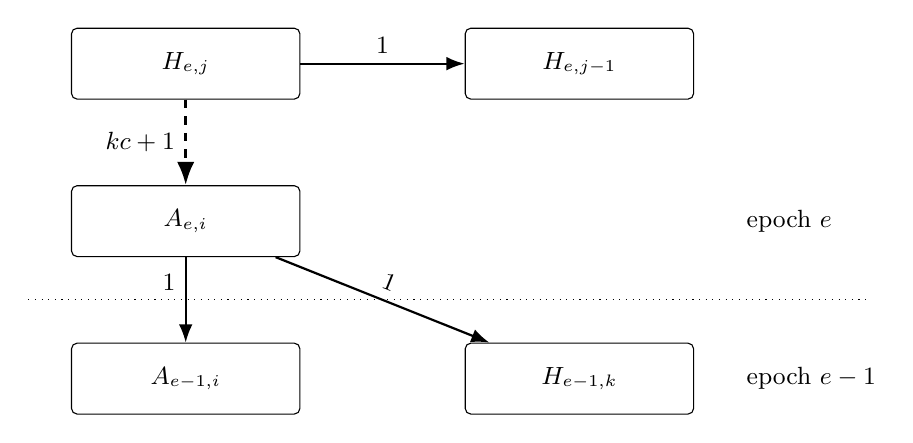
\begin{tikzpicture}[
  >=Latex,box/.style={draw,rounded corners=2pt,minimum width=29mm,minimum height=9mm},
  every node/.style={font=\small},
  cheap/.style={->,thick},
  costly/.style={->,very thick,dashed}
]
\node[box] (h) at (0,2) {$H_{e,j}$};
\node[box] (hp) at (5,2) {$H_{e,j-1}$};
\node[box] (a) at (0,0) {$A_{e,i}$};
\node[box] (ap) at (0,-2) {$A_{e-1,i}$};
\node[box] (oldh) at (5,-2) {$H_{e-1,k}$};
\draw[cheap] (h) -- node[above] {$1$} (hp);
\draw[costly] (h) -- node[left] {$kc+1$} (a);
\draw[cheap] (a) -- node[pos=0.3,left] {$1$} (ap);
\draw[cheap] (a) -- node[above,sloped] {$1$} (oldh);
\draw[dotted] (-2,-1) -- (8.7,-1);
\node[anchor=west] at (7,0) {epoch \(e\)};
\node[anchor=west] at (7,-2) {epoch \(e-1\)};
\end{tikzpicture}

\caption{Representative dependencies for \(e\ge1\) and
\(1\le j\le k\). A path may follow preceding histories before entering
\(A_{e,i}\); the omitted extraction edge
\(H_{e,0}\to H_{e-1,k}\) is another route to the preceding epoch.
The weight \(kc+1\) charges the round guess retained in a suspended
frame. Every child of that array word belongs to the preceding epoch,
so the same path cannot retain another round guess in epoch \(e\).
All weights bound suspended storage up to a common polylogarithmic factor.}
\label{fig:epoch-path}
\end{figure}

\begin{lemma}
\label{lem:epoch-weight}
Every dependency path from the final history has weight
\[
 O(E(k+kc+1))=O(Ek\log(T+2)).
\]
\end{lemma}

\begin{proof}
In epoch \(e\), a path takes at most \(k\) preceding-history edges.
It may then use the extraction edge from \(H_{e,0}\), or enter a
start-array word \(A_{e,i}\) and pay \(kc+1\).
For \(e>0\), that array word has children only \(A_{e-1,i}\) and
\(H_{e-1,k}\); for \(e=0\), it is a base word.
Thus a path has at most one expensive edge and a constant number of
ordinary edges in each epoch. Paths entering an epoch at an array
word satisfy the same bound. Summing over the epochs proves the
claim. Sequential repetitions and reverse calls follow the same
dependencies and do not increase the maximum active path weight.
\end{proof}

\begin{proof}[Proof of Theorem~\ref{thm:main}]
Apply Lemma~\ref{lem:weighted-evaluation} to the base, checkpoint,
extraction and factored history words.
The concrete width in \eqref{eq:word-width} covers each block and
history, and \(g=kc\le d\) because \(b=k^2\ge k\). The word count
\(E(N+k+1)\) is polynomial in \(T\) by \eqref{eq:block-count} and the
chosen parameters. Ordinary fan-in is at most two, so the evaluator
uses three vector registers. For this offset one may compute and supply
the degree bound
\[
 \Delta=(N+1)d
 =O((T+b+1)\log(T+2))=T^{O(1)},
\]
which covers the ordinary degree \(d\) and every history degree.
The candidate count \(2^{kc}\) and the Boolean lookup enumerations
affect time, not this degree or the number of word identifiers.
Base coordinates are fixed controller bits or use the accessor or
filler. Extraction and appending copy fixed slices, and each replay
uses one block and at most \(b+1\) controller slices. The local
Boolean kernels therefore use
\(O(d\polylog T)\) local space and make no word-evaluation calls.
The preceding navigation description supplies the required uniformity.
\mbox{Lemmas~\ref{lem:factored-history} and~\ref{lem:epoch-weight}} verify
the remaining hypotheses. Starting with a zero target yields
the final history, hence its final controller, in space
\[
 \softO(d+Ek)=
 \softO\!\left(b+(1+T/b^2)k\right)
 =\softO(T^{2/5}).
\]
The register pool, reusable local workspace and suspended stack are
all counted. In particular, the current unsuspended guess is included
in the word-sized local term, and no array of checkpoints is materialized.
Trying the offsets reuses this storage, and a completed offset
exists. Reading its finite-control state and halt/timeout flags gives
the required capped outcome.

For the unknown-running-time clause, the access condition holds for
\((x,T)\) at every \(T\ge2\), so it applies separately to all trials
with caps \(2,4,8,\ldots\). Continue after a timeout and return only on
an actual halt. If the machine halts in \(t\) steps, the first sufficient
cap is at most \(2\max(t,2)\). Each trial restarts from the same
cap-independent initial symbols, using its own represented blocks, and
discards its workspace before the next. This gives the asserted bound.
\end{proof}

\begin{remark}
\label{rem:output}
A specified bit of a sequential write-only output can also be
computed: keep its index, an output counter and the monitored bit in
the controller. For indices in the capped output range this costs
\(O(\log(T+2))\) bits. Enlarge \(c\) by these fields and use the same
width formula \eqref{eq:word-width}; the estimates are unchanged.
This does not require storing the output stream or change which
writable block a visit accesses.
\end{remark}

\subsection{What varying the three scales achieves}
\label{sec:balance}

Let the block width be \(B\), epoch length in visits be \(L\), and
round length be \(q\). Ignoring rounding and logarithms, a block
contributes \(B\) bits and the complete epoch transcript contributes
\(L\) bits to the materialized word size \(B+L\). There are
\(T/(BL)\) epochs and \(L/q\) rounds per epoch. The preceding-history
edges therefore contribute \(T/(Bq)\) to the weighted stack, while
one suspended \(q\)-controller guess per epoch contributes
\(Tq/(BL)\). Thus the stack estimate is
\[
 \frac{T}{BL}\left(\frac Lq+q\right)
 =\frac{T}{Bq}+\frac{Tq}{BL}.
\]
At \(q\simeq\sqrt L\), this becomes \(2T/(B\sqrt L)\).
If both \(B,L\le S\), it is at least \(2T/S^{3/2}\).
Balancing this displayed estimate with storage \(S\) therefore gives
the two-fifths exponent. Boundary and ceiling terms are nonnegative
and do not improve this balance. This calculation concerns this
estimate only: it rules out neither improved accounting nor another
transcript or simulation method.

\section{A fixed-multitape comparison}
\label{sec:multitape}

The single selected block in Lemma~\ref{lem:visits} is essential to
the factored round rule. For example, a joint transition inspecting
two independently supplied bits may produce a specified outgoing
controller precisely when the bits are equal. The successful pairs
\(\{00,11\}\) cannot be a product of predicates on the individual
bits. An initial visit supplies this obstruction even with the full
earlier short history fixed.
This observation concerns this factorization, not the possibility
of other multitape simulation methods.

For completeness, the ordinary-rule part of
Lemma~\ref{lem:weighted-evaluation} gives the following comparison.
Here the access condition of Section~\ref{sec:introduction} has a tag
for each initial writable tape and each read-only head, with coordinates
measured from their fixed origins.

\begin{proposition}
\label{prop:multitape}
Fix a deterministic machine with a fixed number of ordinary writable
tapes and read-only input heads, unit movement and fixed origins for
all heads, cap-independent symbol functions, and a fixed accessor.
For every public input \(x\) and supplied binary cap \(T\ge2\) satisfying
the access condition, its finite-control and halting outcome admits a
deterministic simulation
in \(\softO(\sqrt T)\) work-space bits, excluding read-only input storage.
Simulation time is unrestricted.
\end{proposition}

\begin{proof}
If there are no writable tapes, a direct capped simulation stores the
finite-control state, elapsed time, terminal flags, and the fixed number
of read-only head displacements. Unit movement keeps every query within
the cap radius, so the controller and accessor use \(\polylog T\) work bits.
Hence assume the writable-tape count \(m\) is positive, and let
\(b=\lceil\sqrt T\rceil\). On each writable tape, use the represented
blocks of Lemma~\ref{lem:visits}: they contain the real symbols within
distance \(T\) of that tape's origin and a fixed filler outside.
All block words below refer to this represented computation.
The confinement argument applies to every head of every accepted
candidate controller. From elapsed time \(\tau\) and displacement at
most \(\tau\), after \(s\le T-\tau\) further unit steps its displacement
is at most \(\tau+s\le T\). Thus a joint visit never reads or writes an
exterior writable cell, and all read-only queries satisfy the access
condition. Invalid or terminal controllers make no underlying tape query.
The represented and real capped controller trajectories therefore agree.

Apply a common trial offset to all tapes.
The sum of crossing counts, averaged over offsets, is at most
\(mT/b\). End a joint visit when any writable head crosses, or on
halt/timeout. Some offset therefore needs at most
\(R=\lceil1+mT/b\rceil\) visits. A joint visit reads and updates
only its \(m\) selected blocks and is computable in
\(O((mb+1)\polylog T)\) space on those explicit blocks, including
public-symbol access.

For each offset, enumerate a complete list of \(R+1\) raw fixed-width
controller strings, including the prescribed initial one. Hold this list
in one global \(O(R\log(T+2))\)-bit buffer.
For a candidate list \(z_0,\ldots,z_R\), let \(Q_{t,h}\) denote
the block word produced after visit \(t\) for the block on tape \(h\) selected
by the incoming controller \(z_{t-1}\).
Its incoming block is the output \(Q_{s,h}\) from the last earlier
visit \(s<t\) selecting that same tape/block, or the initial block
if none exists. Each \(Q_{t,h}\), and each gate computing or checking
the outgoing controller, depends on at most \(m\) incoming block
words and the prescribed controller \(z_{t-1}\).
The last-update index is found by scanning the retained list.
All dependencies decrease visit number, so their depth is \(O(R)\),
even for malformed lists.

Use the same total parsing convention as in Lemma~\ref{lem:visits},
with a designated valid block on each tape for an invalid controller.
Each transition check compares its deterministic raw outgoing controller
bit for bit with the proposed string \(z_t\).
Apply the ordinary-rule evaluator with word width \(O(b)\), fixed
fan-in and path weight \(O(R)\).
Evaluate the transition checks one at a time. Induction from the
initial controller proves that a passing list is exactly the actual
capped computation: the last-update rule supplies each true
incoming block, and the next check forces the true outgoing
controller. Require a terminal last controller; disregard
insufficient offsets. A completed actual list exists for a good
offset, with stationary padding after termination.

The controller list is stored once, not copied into recursive
frames. Evaluator storage and that buffer together occupy
\(\softO(b+R)=\softO(\sqrt T)\).
Only the maximum storage over offset/list trials is needed.
\end{proof}

Proposition~\ref{prop:multitape} matches the known square-root
exponent but does not assert the sharper logarithmic factor of
Williams's Theorem~1.1~\cite{Williams2025}.
For a fixed ordinary multitape decider halting within
\(T\ge\max\{n,2\}\) steps on an input of length \(n\), the standard
one-writable-tape conversion halts with the same decision within
\(O(T^2)\) steps. Applying the form of Theorem~\ref{thm:main} without
a supplied running time to that converted decider would give
\(\softO(T^{4/5})\) space in the original time parameter.
This is a running-time comparison for halting deciders.
Thus neither the conversion nor the factorization argument
establishes a new general-multitape exponent.

\section{Time lower bounds from the space hierarchy}
\label{sec:hierarchy}

Theorem~\ref{thm:main} has hierarchy consequences analogous to those
Williams derives from his square-root simulation
\cite[Corollaries~1.2--1.3 and Section~4]{Williams2025}.
Write \(\mathrm{TIME}_{1w,\mathrm{ro}}(t)\) for languages decided in
worst-case \(O(t(n))\) time by the fixed deterministic machine model of
Theorem~\ref{thm:main}: one writable tape and head, unit head movements,
and a fixed number of read-only input heads, with the ordinary
cap-independent input encoding described in Section~\ref{sec:introduction}.
Write \(\mathrm{DSPACE}(s)\) for ordinary deterministic \(O(s(n))\)
work-space bits with an endmarked read-only input tape whose head stays
between the endmarkers. We use the standard
space-constructibility convention that a fixed machine can mark exactly
\(s(n)\) work cells on every input of length \(n\); constant-factor
variants give the same statements.

\begin{corollary}[One-writable-tape separation]
\label{cor:space-hierarchy}
For every space-constructible \(s(n)\ge n\) and every fixed
\(0<\epsilon<5/2\),
\[
 \mathrm{DSPACE}(s(n))\not\subseteq
 \mathrm{TIME}_{1w,\mathrm{ro}}\!\left(s(n)^{5/2-\epsilon}\right).
\]
\end{corollary}

\begin{proof}
Set \(a=5/2-\epsilon\) and
\[
 \beta=\frac25\max\{1,a\}
       =\max\left\{\frac25,1-\frac{2\epsilon}{5}\right\}<1.
\]
On an input of length \(n\), compute \(n\) with a logarithmic-space
counter and try doubling caps starting at \(T_0=\max\{2,n\}\), reusing
space after each timeout and returning only on a halt. At every trial
cap \(T\ge n\), rescanning supplies every symbol within the cap radius
in \(O(\log(n+2)+\log(T+2))=O(\log(T+2))\) work bits. Thus the access
condition holds for each capped call, even when \(a<1\).
For a run of length \(t\), the final cap is at most
\(2\max\{2,n,t\}\). Theorem~\ref{thm:main} therefore gives, for any
fixed machine with \(t(n)=O(s(n)^a)\), a uniform deterministic simulation
whose work-space usage in bits satisfies
\begin{align*}
 \text{space}
 &=O\!\left((n+t(n)+2)^{2/5}\log^C(n+t(n)+2)\right)\\
 &=O\!\left(s(n)^\beta\log^{C'}(s(n)+2)\right).
\end{align*}
This includes the length counter. No value of \(s(n)\) or running-time
bound is needed by the simulator.

Choose one \(q\) with \(\beta<q<1\). Every fixed logarithmic exponent
and constant in this bound is absorbed by \(s(n)^q\), so
\(\mathrm{TIME}_{1w,\mathrm{ro}}(s^a)\) is contained in
\(\mathrm{DSPACE}(\lceil s^q\rceil)\). The deterministic space hierarchy,
in its standard constant-factor form, separates
\(\mathrm{DSPACE}(s)\) from \(\mathrm{DSPACE}(r)\) whenever the larger
bound \(s\ge n\) is space-constructible and \(r=o(s)\); constructibility
of \(r\) is not required \cite[Theorem~3.1]{LadnerLynch1976}.
For this application, the passage from the cited exact-cell theorem
to bit-space bounds can be seen directly. Choose \(q'\) with
\(q<q'<1\). After a fixed normalization of the machine and constructor
models, an exactly constructible cell bound \(S=\Theta(s)\) is available,
and each fixed \(O(s^q)\)-bit decider uses
\(O(s^q+\log(n+2))=o(S^{q'})\) cells. For each such decider, the bound
\(\lceil S^{q'}\rceil\) therefore holds at all sufficiently large lengths;
the finitely many exceptional inputs can be handled in finite control.
Apply the exact-cell theorem with
the smaller bound \(\lceil S^{q'}\rceil=o(S)\), which need not be
constructible. Its separating machine uses \(O(S)=O(s)\) bits.
This proves the required separation from
\(\mathrm{DSPACE}(\lceil s^q\rceil)\).
\end{proof}

For a concrete example, fix a standard binary encoding of deterministic
machines \(M\) with one endmarked read-only input tape whose unit-movement
head stays between the endmarkers, one initially blank work tape over a
fixed binary-plus-blank alphabet with one unit-movement head, and an
explicit finite-control transition
table. Use a tuple encoding that stores its
fields verbatim with linear overhead and whose field symbols are
obtainable with logarithmic-space counters. Let \(H\) consist of the
encodings \(\langle M,x,1^k\rangle\)
such that \(|M|\le k\) and \(M(x)\) halts after visiting at most \(k\)
work cells; malformed codes are outside \(H\).

\begin{corollary}[Bounded-space halting]
\label{cor:bounded-space-halting}
The language \(H\) is complete for \(\mathrm{DSPACE}(n)\) under
logarithmic-space many-one reductions of linear output length.
If \(N\) denotes its input length, then for every fixed
\(0<\epsilon<5/2\),
\[
 H\notin
 \mathrm{TIME}_{1w,\mathrm{ro}}\!\left(N^{5/2-\epsilon}\right).
\]
\end{corollary}

\begin{proof}
For membership in linear space, first reject any malformed tuple or transition
table, and reject if \(|M|>k\). A universal simulation then stores the
bounded work interval, head positions and state in
\(O(k+|M|+\log(N+2))=O(N)\) bits, looking up transitions by rescanning
the code. For fixed encoding constants \(K_0,K_1\), the number of bounded
configurations is at most
\[
 K_0(N+2)2^{|M|}(k+1)^3 3^k
 \le 2^{K_1(k+|M|+\log(N+2)+1)}.
\]
The factors account for the bounded input head, state code, work-interval
and head markers, and the fixed three-symbol work alphabet. A conservative
counter for this bound uses \(O(N)\) bits. Reject an attempted visit to a
\((k+1)\)-st work cell, accept a halt within the bound, and otherwise
reject when the clock is exhausted. In the last case a deterministic
bounded configuration has repeated.

Fix \(A\in\mathrm{DSPACE}(n)\). Constant-factor space normalization
gives a fixed decider \(M_A\) in the chosen format using at most \(cn+d\)
work cells. Replace rejection by a stationary loop, leaving acceptance
as a halt, to obtain \(M_A^+\). Choose \(k=c'n+d'\) large enough to
bound this computation and satisfy \(k\ge |M_A^+|\), including small
inputs. Put \(y(x)=\langle M_A^+,x,1^k\rangle\). Then \(x\in A\) if and
only if \(y(x)\in H\), and \(|y(x)|=O(n+1)\).
This is a logarithmic-space reduction of linear output length.
More specifically, given a coordinate \(j\), counters compute the field
boundaries and return a fixed-code, header or unary symbol, or rescan
\(x\) for its indexed bit; outside the encoding they return the prescribed
blank or endmarker. This uses
\(O(\log(n+2)+\log(|j|+2))\) work bits and also computes \(|y(x)|\).
The encoded string \(y(x)\) is independent of the simulation cap.

Suppose a fixed target-model machine decided \(H\) in \(O(N^a)\) time,
where \(a=5/2-\epsilon\). Simulate it on the virtual input \(y(x)\) by
Theorem~\ref{thm:main}, supplying the symbols of its prescribed initial
writable and read-only tapes from \(y(x)\), or the fixed blank symbol,
by the preceding procedure. Start doubling caps at
\(\max\{2,|y(x)|\}\). Since \(|y(x)|\ge n\), symbol access uses
\(O(\log(T+2))\) bits at every coordinate within distance \(T\) of
the fixed head origins, for each trial cap \(T\). Thus every capped call
satisfies the access condition. The last cap is
\(O(n+1+(n+1)^a)\), giving
\[
 O\!\left((n+1)^\beta\log^C(n+2)\right)=o(n),
 \qquad \beta=\frac25\max\{1,a\}<1.
\]
Choosing one \(q\in(\beta,1)\) as above would put every
\(A\in\mathrm{DSPACE}(n)\) in \(\mathrm{DSPACE}(\lceil n^q\rceil)\),
contrary to the space hierarchy. This uses the public-symbol interface
of Theorem~\ref{thm:main}, not closure of one-tape time under
logarithmic-space reductions.
\end{proof}

These are class nonmembership statements in the one-writable-head model,
not lower bounds on every input length. They assert no general multitape
or random-access bound and no logarithmic endpoint.

\bibliographystyle{plain}
\bibliography{references}
\end{document}
